\section{Correction with entanglement}

\subsection{Experimental setup}
We begin with timestamps from a tabletop experiment, where Alice transmits photons to Bob. There is no Doppler shift here, but Bob's signal picks up some noise and losses.

\begin{figure}[ht!]
	\centering
	\begin{subfigure}[t]{0.49\linewidth}
		\centering
		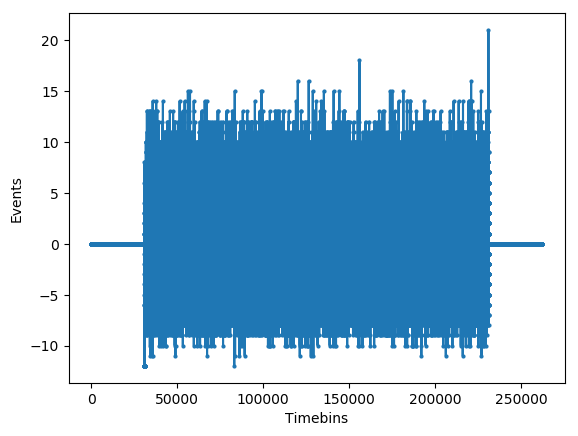
\includegraphics[height=4cm]{assets/aliceBobTimebinAlice.png}
		\subcaption{}
	\end{subfigure}
	\begin{subfigure}[t]{0.49\textwidth}
		\centering
		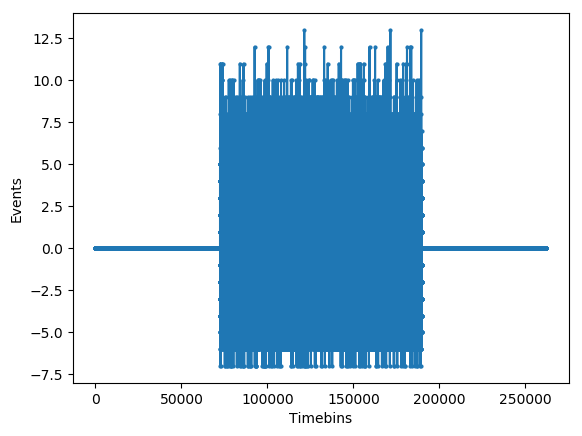
\includegraphics[height=4cm]{assets/aliceBobTimebinBob.png}
		\subcaption{}
	\end{subfigure}
	\caption{Timebins of 10000ns on (a) Alice tabletop atomic clock, (b) Bob tabletop atomic clock}
	\label{fig:timebins}
\end{figure}

To efficiently perform cross-correlation on two-million point dataset, we first use the Fast Fourier Transform with coarse timebins of 10000ns (Fig \ref{fig:FFT}(a)). Having identified a coarse peak, we then zoom in on a window around it and repeat the process with finer timebins (Fig \ref{fig:FFT}(b)). Since the resolution of the timestamps is 2.0ns, we decided on a timebin size of 8.0ns would be precise enough to be useful, yet still robust enough against statistical noise.

\begin{figure}[ht!]
	\centering
	\begin{subfigure}[t]{0.48\linewidth}
		\centering
		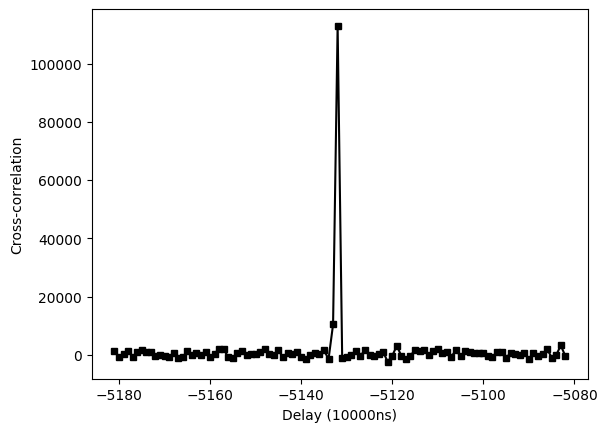
\includegraphics[width=0.97\linewidth]{assets/aliceBobCoarse_cc}
		\subcaption{}
		\label{fig:cc_bin}
	\end{subfigure}
	\begin{subfigure}[t]{0.5\textwidth}
		\centering
		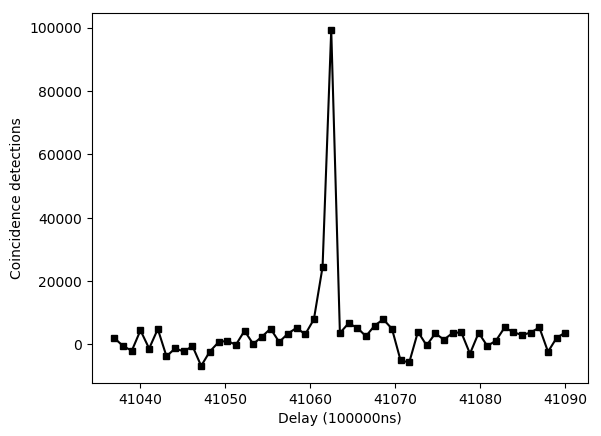
\includegraphics[height=4cm]{assets/aliceBob_cc.png}
		\subcaption{}
	\end{subfigure}
	\caption{Cross-correlation of Alice's and Bob's timestamps, using (a) coarse timebins and FFT, followed by (b) fine timebins with \texttt{pycorrelate}.}
	\label{fig:FFT}
\end{figure}

\subsection{Artificial Doppler shift}
We introduce an artificial Doppler shift on Bob's timestamps. This is done by setting the timestamp to be in a time range for a satellite pass, and calculating the real Doppler shift for each timestamp. We used the \texttt{GALASSIA} satellite (Fig. \ref{fig:TLE}) and the \texttt{pyephem} package for this. 

\begin{figure}[ht!]
\begin{tabular}{ l }
\texttt{GALASSIA }\\
\texttt{1 41170U 15077E   18291.47886069  .00002035  00000-0  73075-4 0  9998 }\\
\texttt{2 41170  14.9881 191.7979 0013088 334.9563  25.0122 15.13422614157130}\\
\texttt{Latitude, longitude, elevation: 1.2954752$^o$, 103.7800079$^o$, 100$^o$ }\\
\texttt{Time and date: 2018/10/19 04:57:11}

\end{tabular}
\caption{GALASSIA TLE and saved pass}
\label{fig:TLE}
\end{figure}

\noindent As expected, the Doppler shift introduces an approximately quadratic delay on the timestamps (Fig. \ref{fig:real_shift}(a)), and it is happening at the steepest rate (\ref{fig:real_shift}(b)). After being shifted, the cross-correlation peak spreads out over several timebins (\ref{fig:real_shift}(c)) and has to be corrected to recover a sharp peak (\ref{fig:real_shift}(d)).

\begin{figure}[ht!]
	\centering
	\begin{subfigure}[t]{0.49\linewidth}
		\centering
		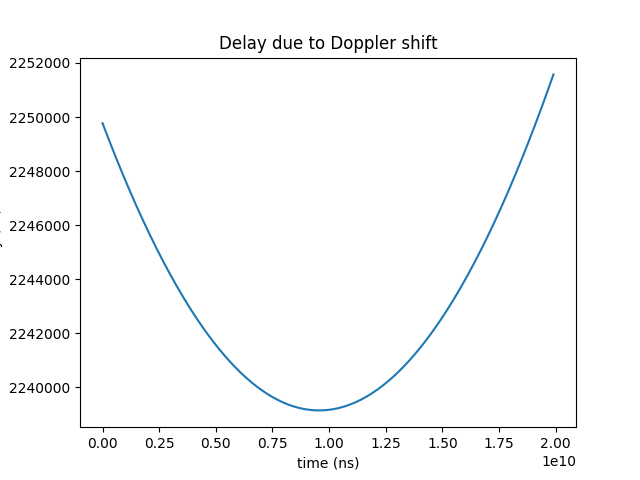
\includegraphics[height=4cm]{assets/delay.png}
		\subcaption{}
	\end{subfigure}
	\begin{subfigure}[t]{0.49\textwidth}
		\centering
		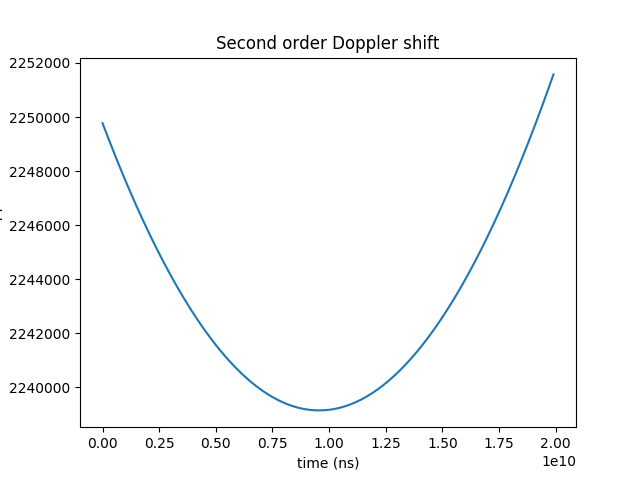
\includegraphics[height=4cm]{assets/range_velocity.png}
		\subcaption{}
	\end{subfigure}
	\begin{subfigure}[t]{0.49\linewidth}
		\centering
		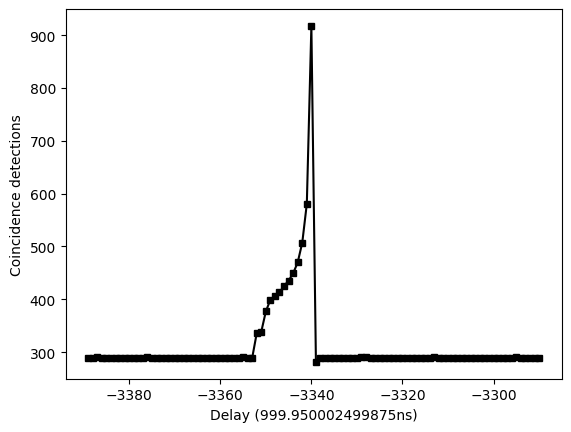
\includegraphics[height=4cm]{assets/propagationDelay_cc.png}
		\subcaption{}
	\end{subfigure}
	\begin{subfigure}[t]{0.49\textwidth}
		\centering
		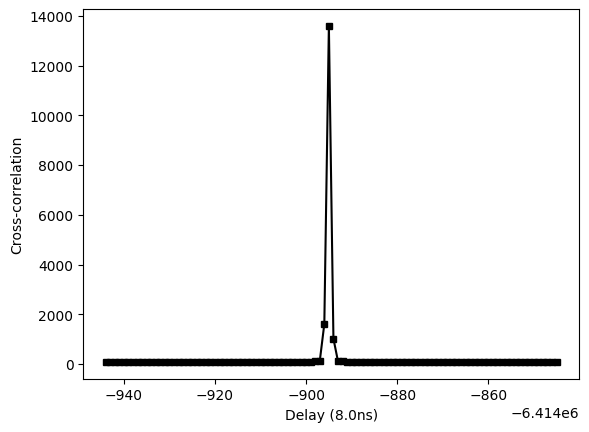
\includegraphics[height=4cm]{assets/propagationDelayGuess_cc.png}
		\subcaption{}
	\end{subfigure}
	\caption{(a) Introduced Doppler shift on each timestamp for the chosen satellite, and (b) rate of change of Doppler shift. (cf. Fig. \ref{fig:doppler_shift}). Cross-correlation of signals with (c) propagation delay and (d) after correction and gradient ascent.}
	\label{fig:real_shift}
\end{figure}

\subsection{Gradient ascent on Doppler shift}

To recover Fig \ref{fig:real_shift}(d) from Fig \ref{fig:real_shift}(c), we use gradient ascent on a guessed Doppler shift function. Our gradient ascent method is as follows:

\begin{enumerate}

	\item Using TLE data and the time range of the satellite pass, guess a Doppler shift as a polynomial function (e.g. quadratic):
	\begin{equation}
		f(x) = ax^2 + bx + c.
	\end{equation}
	Note that we cannot now replicate the exact artificial shift we had put in earlier, since we should not have access to Bob's unshifted timestamps. The point is therefore to recreate the shift as closely as possible using a polynomial fit.
	\item Apply $f(x)$ to Bob's (shifted) timestamps, and perform cross-correlation with Alice's timestamps. 
	\item Define a gain function: here, we want to maximise the total distance between the cross-correlation peak and its adjacent points, i.e. get as sharp a peak as possible: 
	\begin{equation}
		g = 2*\texttt{max(xcorr)} - \texttt{xcorr[maxIdx - 1]} - \texttt{xcorr[maxIdx + 1]}.
	\end{equation}
	This is always positive by definition. We can also normalise the gain function $g' = g / \texttt{max(xcorr)}$. We expect a perfect cross-correlation to have $g' = 2.0,$ with a peak at one point and zero at all others.
	\item Use gradient ascent to update the polynomial coefficients, and maximise the sharpness of the cross-correlation peak:
	\begin{align*}
		a_i &= a_{i-1} + \alpha*\Delta_{a_{i-1}}\\
		b_i &= b_{i-1} + \beta*\Delta_{b_{i-1}},
	\end{align*} 
	where $\alpha, \beta$ are learning rates, and $\Delta_{a_i} = \frac{g_i - g_{i-1}}{a_i - a_{i-1}}, \Delta_{b_i} = \frac{g_i - g_{i-1}}{b_i - b_{i-1}}$ are the gradients which define the direction of the next step. This method treats each coefficient as independent of the others.
	
	For the initial iteration, where there is no previous set of parameters, we use a manual offset to kickstart the ascent. Note also that we ignore the constant offset, since the point of the cross-correlation is to capture that very delay.
	\item Repeat until the gradient ascent no longer improves the result ($g_i < g_{i-1}$). In cases where the learning rate is too low, and our result improves at an ever-slowing rate, we define an $\epsilon$ to terminate the ascent below a certain rate (\texttt{STOP if} $g_i - g_{i-1} < \epsilon$).
	
\end{enumerate}
 